\begin{figure}[h!]
  \centering
  \captionsetup{justification=centering}
  \begin{subfigure}[t]{0.2\linewidth}
    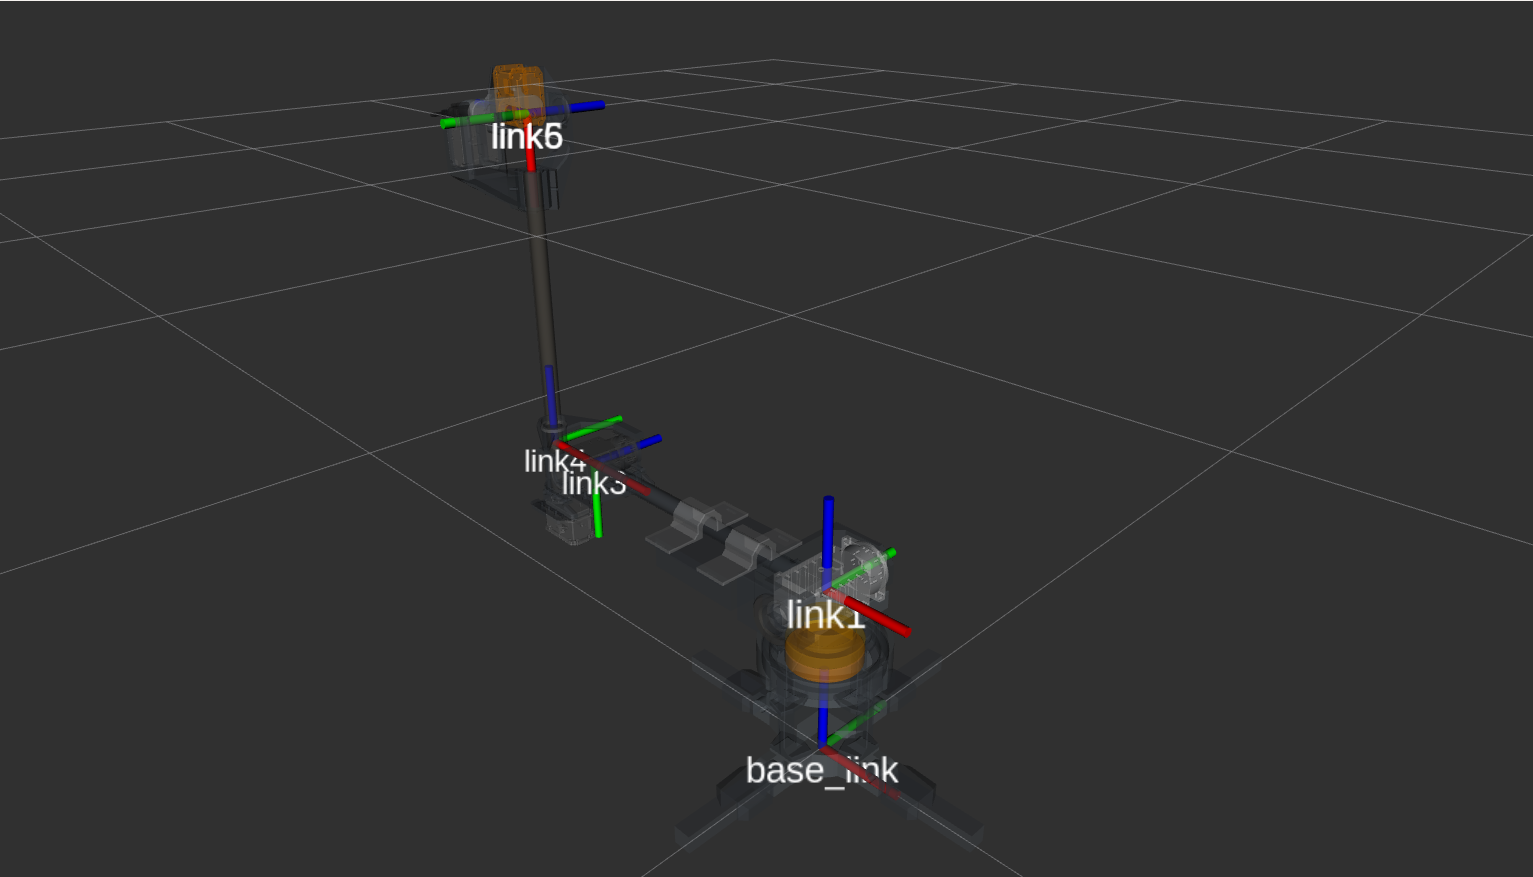
\includegraphics[width=\linewidth]{r_mini_frame1.png}
     \caption{Frame 1}
  \end{subfigure}
  \begin{subfigure}[t]{0.2\linewidth}
    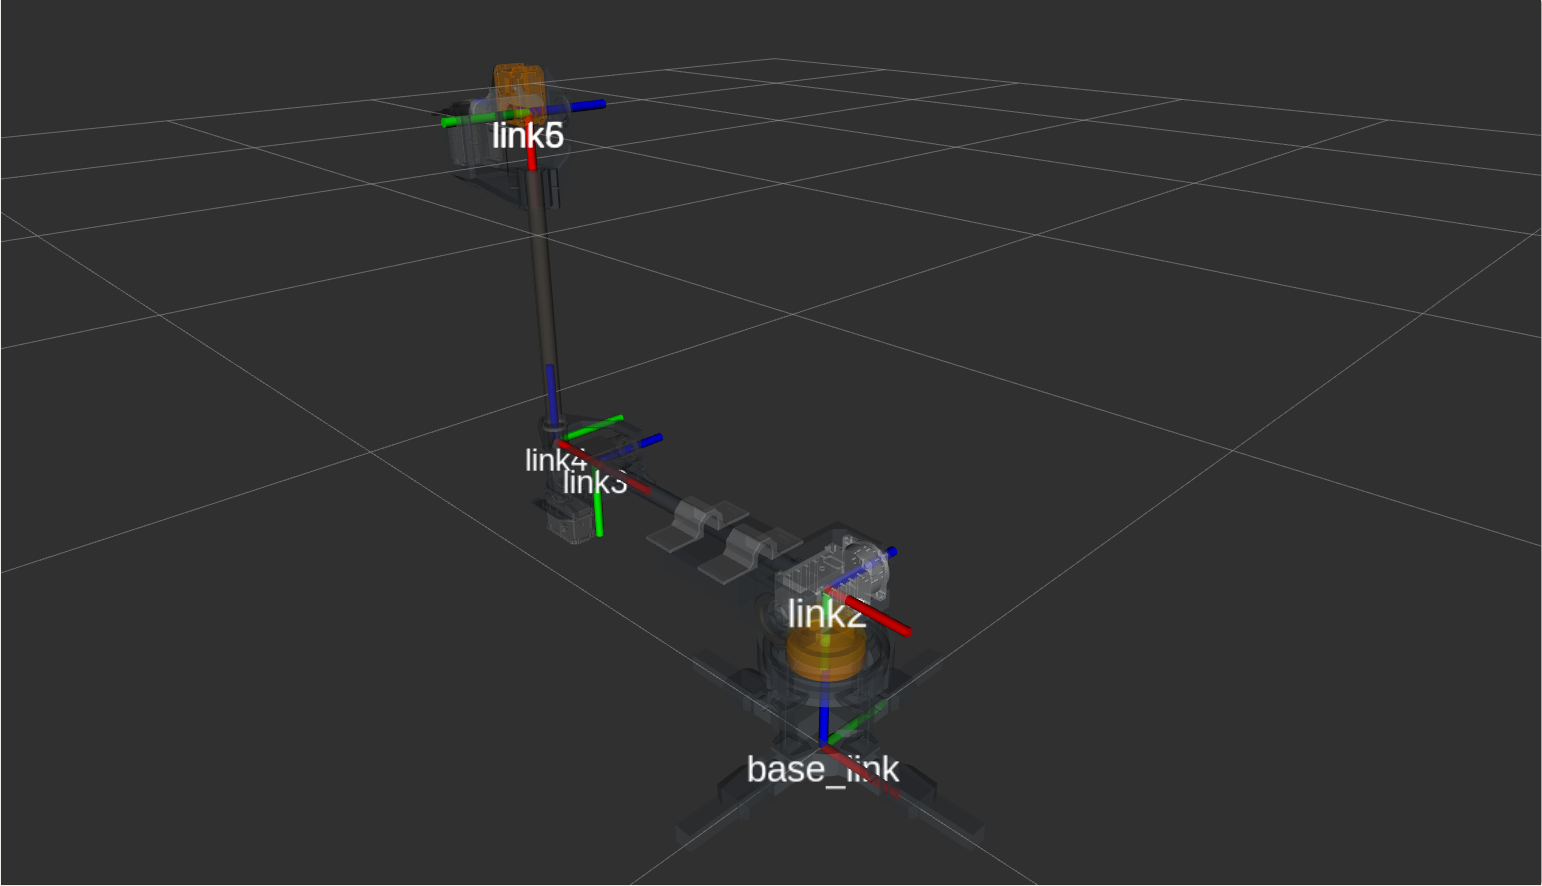
\includegraphics[width=\linewidth]{r_mini_frame2.png}
    \caption{Frame 2 sharing origin with Frame1}
  \end{subfigure}
  \begin{subfigure}[t]{0.2\linewidth}
    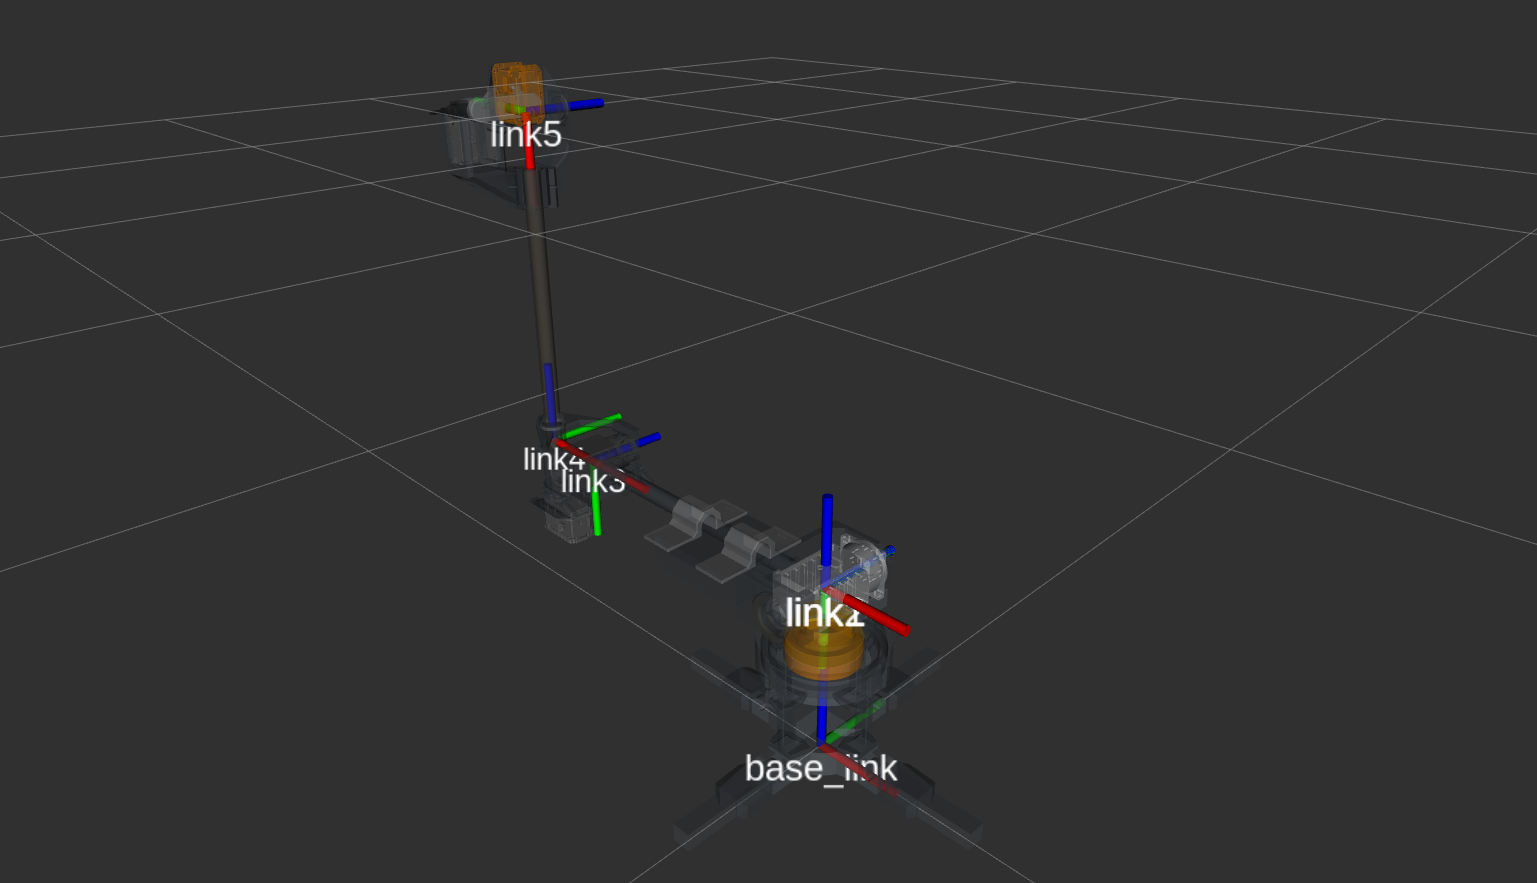
\includegraphics[width=\linewidth]{r_mini_frame5.png}
    \caption{Frame 5}
  \end{subfigure}
  \begin{subfigure}[t]{0.2\linewidth}
    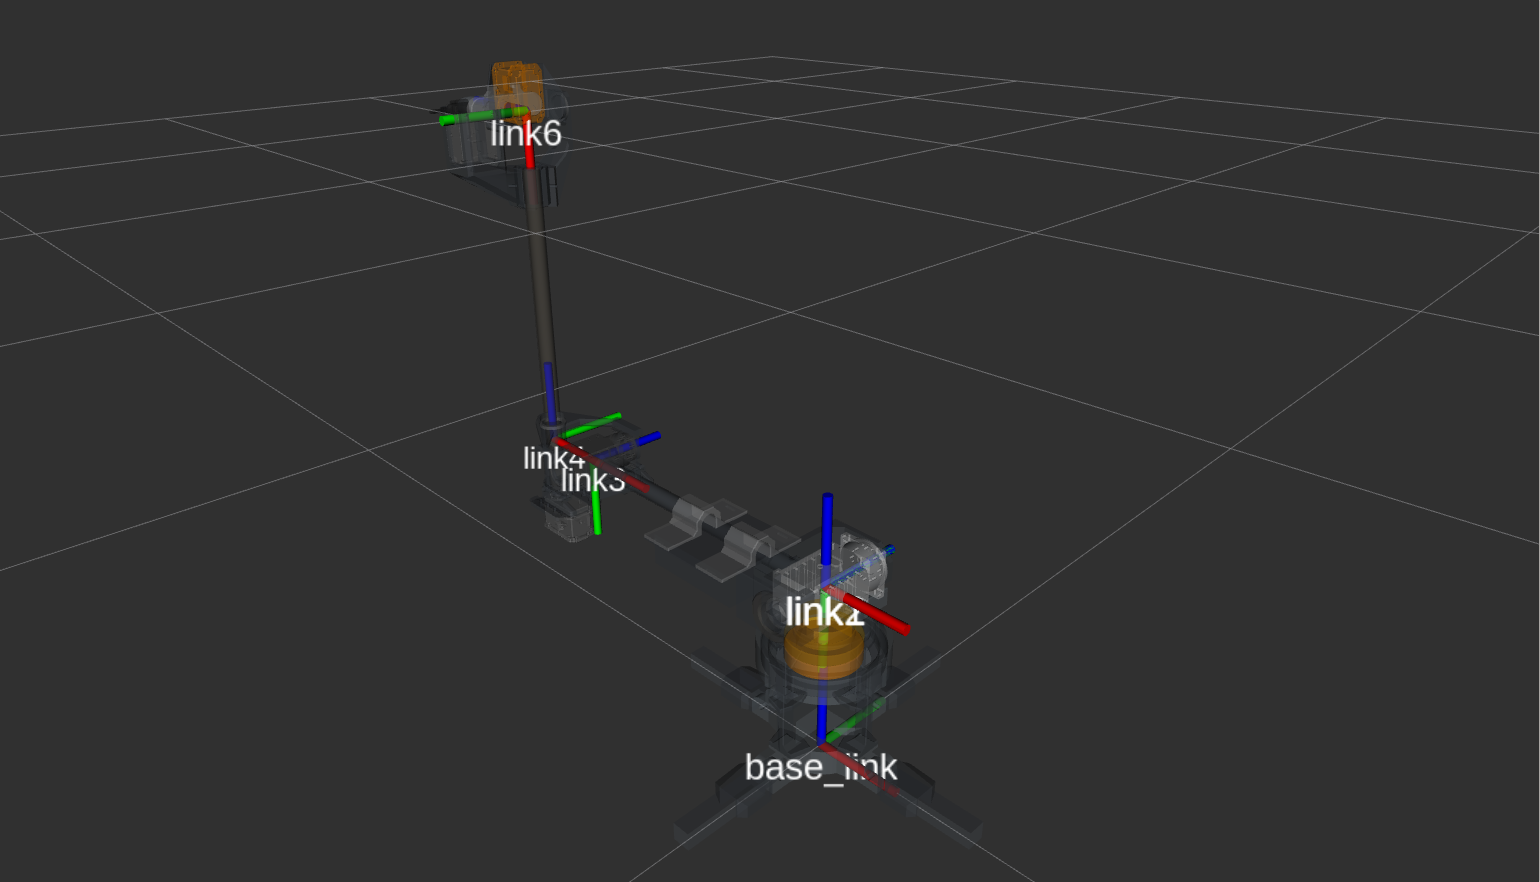
\includegraphics[width=\linewidth]{r_mini_frame6.png}
    \caption{Frame 6 sharing the origin with frame 5}
  \end{subfigure}
  \begin{subfigure}[b]{0.4\linewidth}
    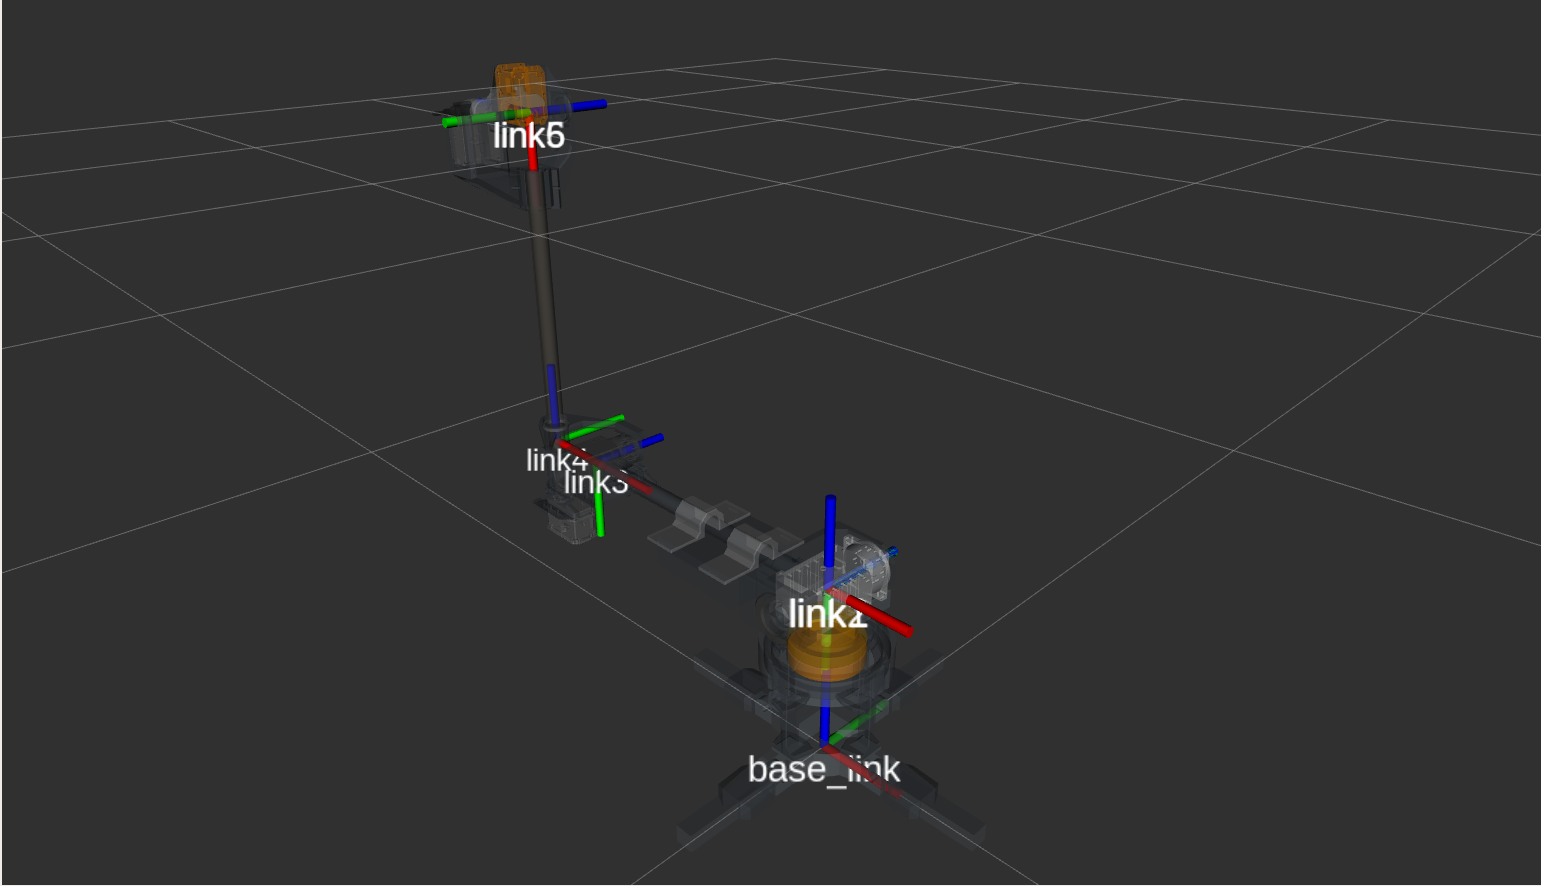
\includegraphics[width=\linewidth]{r_mini_local_frames.png}
    \caption{Rimini build completion.}
  \end{subfigure}

\caption{The location and orientation of \rimini~. The choice of the orientation for each frames are based on Denavit-Hartenberg.
          The joints are values represented by the angle between two $\mathsf{x-axes}$ around the $\mathsf{z-axis}$ or rotation axis of each actuators }
  \label{fig:rimini_joints}
\end{figure}
